\documentclass[12pt,tikz,border=0pt]{standalone}
\usetikzlibrary{shapes.geometric,backgrounds,calc}

\begin{document}

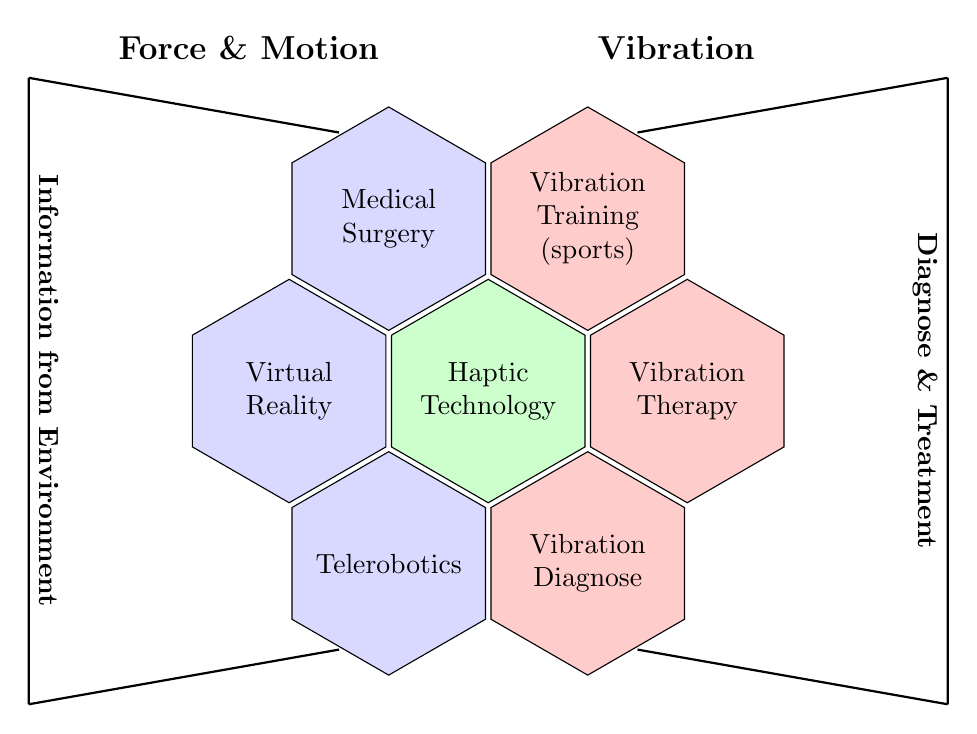
\begin{tikzpicture}[
%	yscale=1.2,
    hexag/.style={
	    draw,
	    shape=regular polygon,
	    regular polygon sides=6,
%	    minimum size=30mm,
        inner sep=-8pt,
        outer sep=1pt, %Adjust for different separations of cells
        text width=23mm,
        align=center,
%        font={\sffamily,\bfseries},
%        fill=white,
	    shape border rotate=90,
	    transform shape=true,
    },
]

\def\AN{10}         %angle of wings
\def\LS{4}          %length of wings
\def\COR{red!20}    %color of right parts
\def\COL{blue!15}   %color of left parts

\node[hexag,fill=green!20] (centro) at (0,0) {Haptic Technology};
\node[hexag,anchor=180,fill=\COR] (A) at (centro.0)   {Vibration Therapy};
\node[hexag,anchor=240,fill=\COR] (B) at (centro.60)  {Vibration Training (sports)};
\node[hexag,anchor=300,fill=\COL] (C) at (centro.120) {Medical Surgery};
\node[hexag,anchor=0  ,fill=\COL] (D) at (centro.180) {Virtual Reality};
\node[hexag,anchor=60 ,fill=\COL] (E) at (centro.240) {Telerobotics};
\node[hexag,anchor=120,fill=\COR] (F) at (centro.300) {Vibration Diagnose};

\draw[thick] (B.side 5) -- ++( \AN:\LS) coordinate (X);
\draw[thick] (F.side 3) -- ++(-\AN:\LS) coordinate (Y);
\draw[thick] (X) -- (Y) node [midway, below,sloped] {\bfseries Diagnose \& Treatment};

\draw[thick] (C.side 6) -- ++(180-\AN:\LS) coordinate (X);
\draw[thick] (E.side 2) -- ++(\AN-180:\LS) coordinate (Y);
\draw[thick] (X) -- (Y) node [midway, above,sloped] {\bfseries Information from Environment};

\coordinate (P1) at (C.north);
\coordinate (P2) at (B.north);

\node [anchor=east, yshift=20pt] at (P1) {\bfseries \large Force \& Motion};
\node [anchor=west, yshift=20pt] at (P2) {\bfseries \large Vibration};

%Uncomment below if you want connecting lines in the background
\begin{scope}[on background layer]
\draw[thick] 
%			 (B.side 5) -- (centro.center) -- (F.side 3)
%			 (C.side 6) -- (centro.center) -- (E.side 2)
% 			 (D.center) -- (A.center)
			 ;
\end{scope}


\end{tikzpicture}
\end{document}\grid
